\chapter{Grundlagen}\label{ch:related_work}
%alles was man braucht um den Rest zu verstehen
In dem folgenden Kapitel werden Technologien und Konzepte vorgestellt die für das  Verständnis der Arbeit erforderlich sind. Es wird angenommen das der Leser über grundlegendes Verständnis der Funktionsweise des Internets und der Webentwicklung verfügt.

\section{Ressourcen}
%\subsection{Statische Ressourcen}
Unter statischen Ressourcen werden im Rahmen dieser Arbeit Inhalte einer Website verstanden, die für alle Nutzer gleich sind. Sie sind im Gegensatz zu dynamischen Inhalten nicht nutzerspezifisch und können daher gut über ein CDN (siehe \ref{cdn}) verteilt werden. Insbesondere die so genannten Assets einer Internetseite sind meist statisch. Dies sind meist Javascript- und CSS-, aber auch Bild-Dateien. Auch Videos fallen häufig in diese Kategorie.

%\subsection{Dynamisch generierte Ressourcen}

Im Gegensatz zu statischen Ressourcen werden im Kontext dieser Arbeit Inhalte als dynamisch generiert bezeichnet, wenn sie zur Laufzeit der Website erzeugt werden. Dabei lässt sich zwischen nutzergenerierten Inhalten und automatisch generierten Inhalten, z.B. Statistiken, unterscheiden.

Dynamische Inhalte können nutzerspezifisch sein, in diesem Fall werden jedem Nutzer bei selber Abfrage andere Inhalte angezeigt.

\section{\cdn} \label{cdn}
Unter einem \cdn, auch Content Delivery Network, versteht man ein Netzwerk, in dem sich Clients Inhalte von einer Reihe von Knoten laden. Ein \cdn stellt dem Nutzer Auslieferungs- und Speicherkapazitäten zur Verfügung. Dadurch kann die Last auf dem Ursprungsserver und die Latenz auf Seiten der Nutzer reduziert werden. Die reduzierten Ladezeiten werden unter anderem durch eine bessere geographische Nähe und damit geringere Netzlaufzeiten erreicht.

Es lassen sich drei Klassen von \cdns unterscheiden. Infrastrukturbasierte CDN, die auf einer geografisch verteilten Serverinfrastruktur basieren, \pTp-basierte \cdns bei denen die Inhalte direkt zwischen den Teilnehmern verteilt werden, und hybride \cdns die auf einer Kombination aus Serverinfrastruktur und \pTp-Verteilung beruhen.

%- Content Distribution Network
%- Servernetzwerk das inhalte lokal verteilt
%- reduzierung der physischen Entfernung
%- bereitstellung von auslieferkapazitäten
\subsection{Infrastrukturbasierte-\cdns}
Infrastrukturbasierte \cdns bestehen aus einem Ursprungsserver, der von dem Bereitsteller der Inhalte kontrolliert wird, und einem Netzwerk aus Replikatservern. Die Replikatserver übernehmen die Verteilung der Inhalte an die Clients. Sie fungieren als ein möglichst regionaler Cache, in dem Inhalte des Ursprungsservers gespiegelt werden. Ein Distributionssystem ist dafür verantwortlich die Inhalte auf den Replikaten zu aktualisieren und übernimmt das Routing bei einer Anfrage eines Clients. Unter Zuhilfenahme verschiedener Metriken versucht das Distributionssystem, einen möglichst optimalen Replikatserver für den Client zu finden. Diese Metriken unterscheiden sich zwischen den Anbietern. Häufig werden jedoch geografische Entfernung, Latenzzeiten und die Übertragungsrate berücksichtigt. Um eine möglichst geringe Latenz zu erreichen, sind infrastrukturbasierte \cdns häufig geografisch sehr verteilt und bestehen aus mehreren tausend Replikaservern. So besitzt Akamai, einer der größten \cdn-Anbieter, über 137000 Server in 87 Ländern. \cite{akamaiPeer} 

%-ein ursprungsserver
%- viele replicaserver
%- request routing system wählt optimalen replica server
%- ua. nach geographische Entfernung, Latenzzeit, Übertragungsrate
%137,000 servers in 87 countries
%within over 1,150 Internet networks, \cite{akamaiPeer}

%https://de.wikipedia.org/wiki/Content_Delivery_Network
\subsection{\pTp-basierte \cdns }

Bei einem \pTp-basierten \cdn laden \clients Inhalte nicht von einem Ursprungsserver, sondern von einem anderen \client. Dazu bilden sie Overlay-Netzwerke und setzen Techniken von \pTp-Netzwerken zum Auffinden von Ressourcen ein.(siehe \ref{pTp}) Im Rahmen dieser Arbeit wird zwischen Filesharing-Netzwerken und \cdn-Netzwerken zu unterschieden. Filesharing-Netzwerke, wie z.B. Bittorent\footnote{https://www.bittorrent.com/lang/de/}, zielen auf die Verteilung von Dateien zur späteren Verwendung ab. \cdns wiederum werden unter anderem von Websites zur Auslieferung von statischen Inhalten verwendet. Während es bei Filesharing-Netzwerken akzeptabel sein kann, dass das Auffinden von Ressourcen eine gewisse Zeit in Anspruch nimmt, ist dies bei \cdns nicht der Fall.

%test \cite{p2pBook2005}
% https://de.wikipedia.org/wiki/Peer-to-Peer#Typen_von_Peer-to-Peer-Systemen
%gegenmodell zu client server
%gleichbererchtigte teilnehmer eines rechnernetzwerkes
%overlays erklären??
%häufig aufgabenverteilung der peers
%unstrukturierte p2p:
%	keine peer objekt zuordnung
%	zentralisierte p2p netzwerke - server zur verwaltung
%	reine p2p netzwerke - keine verbindung zu unbekannten ips
%	hybride p2p n. mehere zentrale server die dynamisch zugeteilt werden
%	zenralisierte und reine p2p netzwerke 1.gen. 
%strukturierte p2p:
%	objektzuordnung vorhanden --> suche möglich
%	oft verteilte hashtabellen --> verteilter index

%Peers weisen eine hohe Heterogenität bezüglich der Bandbreite, Rechenkraft, Online-Zeit, … auf.
%Die Verfügbarkeit und Verbindungsqualität der Peers kann nicht vorausgesetzt werden („Churn“).
%Peers bieten Dienste und Ressourcen an und nehmen Dienste anderer Peers in Anspruch (Client-Server-Funktionalität).
%Dienste und Ressourcen können zwischen allen teilnehmenden Peers ausgetauscht werden.
%Peers bilden ein Overlay-Netzwerk und stellen damit zusätzliche Such-Funktionen zur Verfügung.
%Peers haben eine signifikante Autonomie (über die Ressourcenbereitstellung).
%Das P2P-System ist selbstorganisierend.
%Alle übrigen Systeme bleiben konstant intakt und nicht skaliert.
\subsection{Hybride \cdns}
Hybrid \cdns kombinieren \pTp-\cdns und infrastrukturbasierte \cdns. Bei hybriden \cdns wird zuerst versucht, die Resource über das Peer-Netzwerk zu laden. Ist dies nicht möglich, wird auf ein infrastrukturbasiertes \cdn zurückgegriffen. Dadurch kann die Last auf dem \cdn verringert und durch die Kombination verschiedener \cdns eine bessere Ausfallsicherheit erreicht werden. Häufig kommt diese Art der \cdns zum Einsatz wenn Ressourcen für Websites mit einem \pTp-Ansatz verteilt werden sollen. Da in diesem Kontext nicht alle Teilnehmer die technischen Voraussetzungen mitbringen, um an dem \pTp-Netzwerk teilzunehmen, ist eine entsprechende alternative Lösung nötig. Da viele Websites bereits mit einem infrastrukturbasierten \cdn arbeiten, liegt nahe, dieses weiter zu verwenden.

\section{\pTp-Netzwerke} \label{pTp}
Bei einem \pTp-Netzwerk handelt es sich um eine Netzwerkstruktur, bei der alle Teilnehmer gleichberechtigt sind. Sie bildet damit das Gegenkonzept zur klassischen Client-Server-Struktur, bei der einer oder mehrere Server einen Dienst anbieten, der von Clients genutzt werden kann. In einem \pTp-Netzwerk können die Teilnehmer sowohl Dienste anbieten als auch nutzen. Typische, wenn auch nicht notwendige Charakteristika, sind laut Steinmetz\cite{p2pBook2005}:

\begin{itemize}
  \item Heterogenität der Internetbandbreite der Teilnehmer
  \item Verfügbarkeit und Qualität der Verbindung zwischen Teilnehmern kann nicht vorausgesetzt werden
  \item Dienste werden von den Teilnehmern angeboten und genutzt
  \item Teilnehmer bilden ein Netz, das auf ein bestehendes Netz aufgesetzt wird (Overlay-Netzwerk) und stellen Suchfunktionen bereit
  \item Es besteht eine Autonomie der Teilnehmer bei der Bereitstellung von Ressourcen
  \item Das System ist selbstorganisiert
  \item Die restlichen Systeme müssen nicht skaliert werden und bleiben intakt
\end{itemize}
\pTp-Netzwerke lassen sich einteilen in zentralisierte, reine und hybride \pTp-Netzwerke. Zentralisierte Netze haben zur Verwaltung einen Server, der unter anderem die Verbindung der Teilnehmer übernimmt. Dadurch ist es möglich, eine Verbindung aufzubauen, ohne dass die IP-Adresse im Vorfeld bekannt ist. Reine \pTp-Netzwerke haben keinen zentralen Verwaltungsserver. Die Verwaltung des Netzwerkes wird von den Teilnehmern selber übernommen. Das hat zur Folge, das eine Verbindung nur möglich ist, wenn die IP-Adresse des anderen Teilnehmers bekannt ist. 

Je nachdem, ob die Overlay-Struktur eines \pTp-Netzwerkes hierarchisch ist oder nicht, spricht man von hierarchischen oder nicht hierarchischen \pTp-Netzwerken. Die meisten zentralisierten und hybriden Netzwerke verfügen über eine hierarchische Overlay-Struktur. Hierarchische Overlays bieten gute Skalierbarkeit und Effizienz beim Routing. Reine \pTp-Netzwerke haben häufig eine nicht hierarchische Overlay-Struktur. Nicht hierarchische Netzwerke haben den Vorteil, die Last gut auf viele Peers verteilen zu können und verfügen über eine hohe Ausfallsicherheit.\cite{searchingsurvey}

\pTp-Netzwerke lassen sich des Weiteren nach Datenspeicherort und Netzwerkstruktur in unstrukturierte, lose strukturierte und stark strukturierte Netzwerke unterteilen. \cite{searchingsurvey}

In unstrukturierten \pTp-Netzwerken bestehen keine Regeln dafür, wo Daten gespeichert werden. Die Zuordnung ist willkürlich. Ein Beispiel für diese Art von \pTp-Netzwerken ist das Gnutella Netzwerk.\cite{gnutella} Um ein Objekt zu finden, müssen alle Teilnehmer des Netzwerks gefragt werden. Dadurch steigt die Belastung des Netzwerks mit zunehmender Anzahl an Peers. Um die Last auf Seiten der Peers zu reduzieren, wurden eine Reihe von Algorithmen vorgeschlagen, unter anderem iterative deepening\cite{deepening}, direct BFS\cite{deepening}, intelligent search\cite{intelligentSearch} und locale indices based search\cite{deepening} vorgeschlagen.

In lose strukturierten \pTp-Netzwerken, wie z.B. Freenet\cite{freenet} oder Symphonie\cite{symphonie} bestehen keine strikten Regeln für die Zuordnung. Um das Routing zu beschleunigen, wird mit Hinweisen gearbeitet. So hat Symphonie zwar eine eindeutige Zuordnung von Objekten zu Peers, das Overlay-Netzwerk wird jedoch propabilistisch bestimmt. 

Strukturierte \pTp-Netzwerke, wie Chord\cite{chord} oder Kademlia\cite{kademlia}, haben eine strike Zuordnung von Objekt und Peer, ebenso wie eine eindeutige Festlegung des Overlay-Netzwerkes. Es ist also möglich, gezielt nach einem Objekt zu suchen. Mit Hilfe von verteilten Hash-Tabellen ist das Auffinden von Ressourcen in diesen Netzwerken in logarithmischer Zeit möglich. Bei einer verteilten Hash-Tabelle wird die Routing-Tabelle nicht auf einem Peer oder Server gespeichert, sondern auf die Peers verteilt. Jeder Eintrag der Tabelle wird gehasht, ebenso wie jede Peer-Id. Jeder Peer ist für die Verwaltung einer Teilmenge der Einträge verantwortlich. 

\section{\webrtc Web Real-Time Communication}

\webrtc ist ein offener Standard, mit dem Echtzeitkommunikation zwischen Browser und mobilen Anwendungen ermöglicht wird. Mit Hilfe von \webrtc ist es möglich, eine direkte Verbindung zwischen Browsern aufzubauen und Daten direkt zwischen den Clients auszutauschen, ohne dass externe Plugins erforderlich sind. \webrtc ermöglicht neben dem Austausch von Video- und Audio-Daten auch die Übertragung von Binärdaten.\cite{webrtc-book} Der W3C\cite{w3Webrtc} standardisiert \webrtc und definiert dafür eine Sammlung von APIs und Protokollen.

Aktuell wird \webrtc von Chrome, Firefox, Safari, Android und iOS unterstützt.\cite{caniuse-webrtc}

\subsection{Verbindungsaufbau - Signalling}

\begin{figure}[!h]
	\centering
	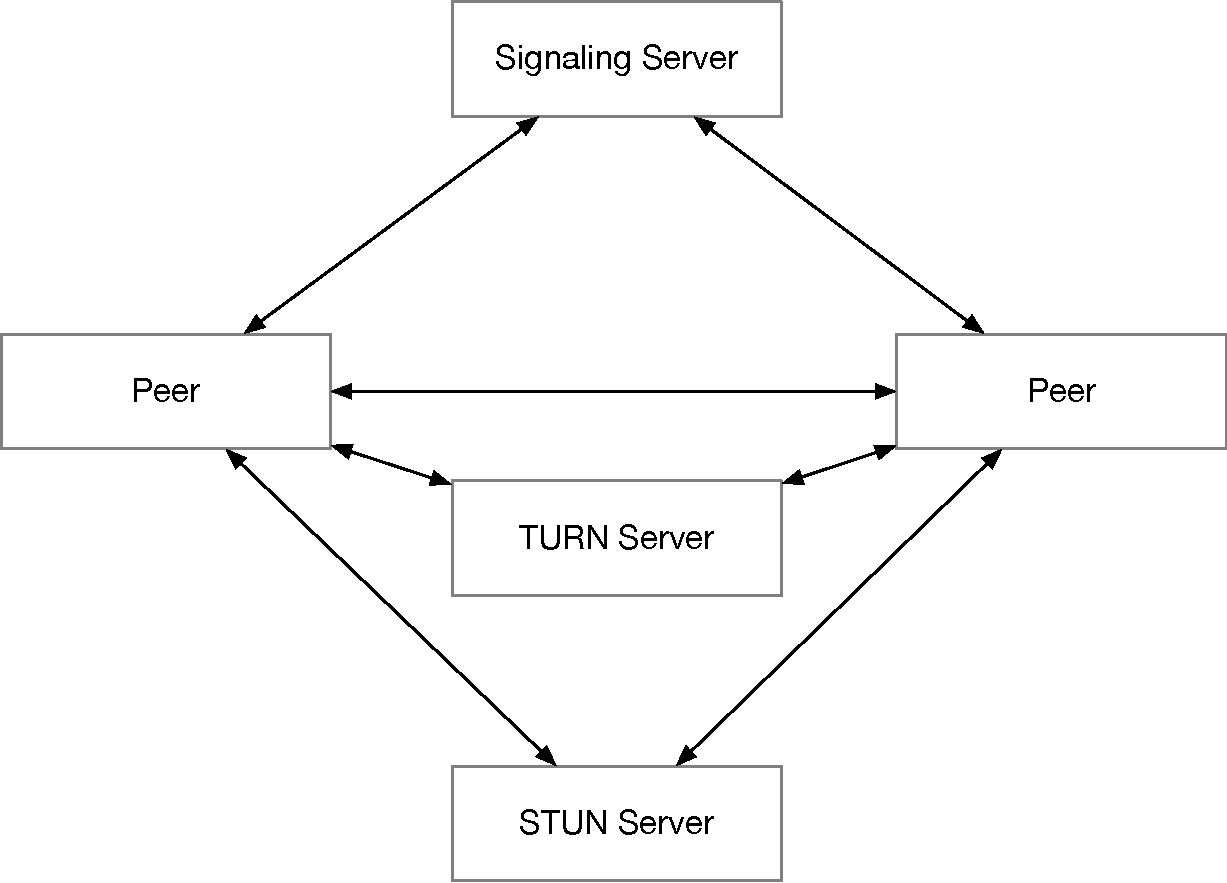
\includegraphics[width=0.8\textwidth]{figures/Webrtc_overview}
	\caption[Überblick Server/Client Struktur Webrtc]{Überblick Server/Client Struktur Webrtc}
	\label{fig:webrtc_overview}
\end{figure}

Damit zwei \clients sich miteinander verbinden können, müssen sie voneinander wissen und Informationen über Metadaten zum Verbindungsaufbau, wie z.B. IP-Adressen und Ports austauschen.

Das Signaling koordiniert die Kommunikation der Verbindungen zwischen Peers. Mit Hilfe des Signalings werden unter anderem die Metadaten ausgetauscht, die benötigt werden, um eine erfolgreiche Webrtc-Verbindung aufzubauen. Dazu wird das SDP-Protokoll verwendet. Unter anderem werden folgende Metadaten ausgetauscht\cite{html5-rocks-signaling}:

\begin{itemize}
	\item Session-Metadaten zum Öffnen/Schließen von Verbindungen
	\item Fehlernachrichten
	\item Metadaten über die zu übertragenden Medien (z.B. Codecs)
	\item Schlüsseldaten für verschlüsselte Verbindungen
	\item Netzwerkdaten, wie öffentliche IP-Adressen und Ports
\end{itemize} 

Der Webrtc-Standard legt keine für das Signaling zu verwendende Technologie oder Protokolle fest, um so die Integration mit bestehenden Technologien zu verbessern und es dem Entwicklern zu ermöglichen, das für den Anwendungsfall beste Protokoll zu verwenden. Allerdings legt er fest, dass eine bidirektionale Kommunikation zwischen den \clients notwendig ist.

%https://www.html5rocks.com/en/tutorials/webrtc/infrastructure/#what-is-signaling
%https://courses.cs.washington.edu/courses/cse522/05au/searchingsurvey.pdf
% For signaling: to enable the exchange of media and network metadata to bootstrap a peer connection.
%
\subsection{STUN-Server}

Da die Anzahl von IPv4 Adressen begrenzt ist, verwenden die meisten Subnetze NATs. Das hat zur Folge, dass diese Clients nicht wissen, über welche IP-Adresse und welchen Port sie wie erreichbar sind. Daher ist der Einsatz von STUN-Servern nötig, um einen Verbindungsaufbau zu ermöglichen. STUN-Server überprüfen eingehende Anfragen auf IP-Adresse und Port und senden diese Informationen zurück an den Client, der somit in der Lage ist, diese Information weiterzureichen und damit auch außerhalb seines lokalen Netzwerkes erreichbar ist. Das STUN-Protokoll ist im RFC 3489\cite{rfcStun} definiert und ist nicht auf Webrtc beschränkt.


%not enough IPv4 addresses
%→ most clients behind NATs, not reachable directly by IP address
%
%client behind NATs can’t know how they can get accessed from the internet
%→ using STUN server
%
%STUN servers check the IP and port of incoming request and send the information back

\subsection{TURN-Server}

Verwaltete Netzwerke, wie die von Unternehmen, haben häufig Firewalls und Port blocking -Systeme installiert, um die Sicherheit des Netzwerks zu gewährleisten. Das kann dazu führen, dass \webrtc-Verbindungen nicht aufgebaut oder Daten nicht über Webrtc-Verbindungen übertragen werden können.

TURN-Server bieten eine Fallback-Lösung für diesen Fall. Sie haben eine öffentliche IP und sind über das Internet erreichbar. Im Fehlerfall kann der Datenverkehr über einen TURN Server geleitet werden, sodass die Kommunikation nicht unterbrochen wird.

\subsection{SDP - Session Description Protocol}
\begin{listing}[h]
	\inputminted{javascript}{listings/sdp_example.txt}
	\caption{Beispiel eines SDP Paketes}
	\label{lst:sdp_example}
\end{listing}
SDP\cite{sdp-standard} wurde zur Verwaltung von Kommunikationssitzungen, wie z.B. SIP entwickelt. Mit Hilfe von SDP werden beim Verbindungsaufbau wichtige Metadaten ausgetauscht. Über SDP-Pakete teilt ein Nutzer einem anderen Nutzer unter anderem verfügbare Codecs, seine IP-Adresse und den zu verwendenden Port mit. Listing \ref{lst:sdp_example} zeigt beispielhaft ein SDP-Paket.


%\begin{itemize}
%	\item Session Description Protocol (SDP, RFC 4566) 
%	\item beschreibt Eigenschaften von Eigenschaften von Multimediadatenströmen
%	\item verwaltet kommunikationssitzungen z.b. SIP(IP-telefonie)
%	\item keine aushandlungsmechaniken sondern nur beschreibungen der Datenströme
%	\item 
%	\item daten aus eigener anwendung einfügen
%	\item Felder beschreiben? zumindest die wichtigesten/verwendeten
%\end{itemize}

\subsection{ICE - Interactive Connectivity Establishment}
Um den Verbindungsaufbau zwischen zwei Clients auszuhandeln, greift Webrtc auf das ICE\cite{rfc-ice} Framework zurück. Aufgrund des begrenzten IPv4-Adressraums verwenden viele Netzwerke NATs. Das hat zur Folge, dass ein Client nicht mehr direkt über seine öffentliche IP-Adresse erreichbar ist. ICE ist dafür zuständig, einen Weg zu finden zwei Peers dennoch zu verbinden. Dazu wird zuerst versucht, eine direkte \pTp-Verbindung mit Hilfe der lokalen IP des Host-Gerätes aufzubauen. Ist dies nicht möglich, wird versucht, mit Hilfe eines STUN Servers die öffentliche IP und den öffentlichen Port zu ermitteln und über diese eine Verbindung zu initialisieren. Schlägt dies ebenfalls fehl, so wird auf einen TURN-Server zurückgegriffen, der als Mittelsmann für die Kommunikation fungiert. Alle drei Verfahren werden parallel angestoßen, um so den effektivsten Weg zu ermitteln. Die bereitgestellten Kandidaten werden nach Priorität sortiert bereitgestellt. Aus allen Kandidaten wird der mit dem geringsten Mehraufwand verwendet.

%setting: 2 peers, signaling server, STUN server
%each peer has a variety of candidate transport addresses (IP:port) 
%addresses from directly attached network (host candidate)
%translated transport (server reflexive) address
%ICE determine  which pairs of addresses work and which connection should be used
%try all possible pairs in smart order

\subsection{Webrtc APIs}
Um eine \pTp Verbindung zu ermöglichen stellt der Webrtc-Standard drei APIs zur Verfügung. Im folgenden wird ein grober Überblick über die APIs gegeben.
\begin{description}
\item[RTCPeerConnection]\hfill \\
Das RTCPeerConnection Interface repräsentiert eine Verbindung vom lokalen \client zu einem anderen \client. Ein RTCPeerConnection-Objekt hält den momentanen Zustand der Verbindung ebenso wie Metadaten über den verbundenen Peer. Sie stellt Funktionen zum Verwalten von Verbindungen bereit.

%\begin{itemize}
%	\item Repräsentiert verbindung zum peer
%	\item Code Beispiel
%\end{itemize}
% RTCPeerConnection is used to connect peers across the internet.


\item[RTCDataChannel]\hfill \\
Die RTCDataChannel API ermöglicht die Übertragung von Text und Binärdaten in Form von Bitstreams. Mit ihr ist es möglich die Datenformate String, Blob, Arraybuffer und ArraybufferView zu übertragen.\cite{rfc-datachannel} Um eine verschlüsselte Übertragung zu ermöglichen, werden Daten mittels SCTP (Stream Control Transmission Protocol) übertragen. SCTP ist ein verbindungsorientiertes Protokoll mit Unterstützung für Multistreaming.\cite{rfc-sctp} 

RTCDataChannel stellen mehrere Übertragungsmodi zur Verfügung. Wird ein Datachannel als Reliable initialisiert, so wird garantiert, dass der Empfänger die Nachricht erhält. Ist dies nicht erforderlich, so kann ein Datachannel als Unreliable initialisiert werden. Dadurch entsteht weniger Mehraufwand und die Übertragung wird beschleunigt. Wird ein Datachannel als Ordered initialisiert, so wird nicht nur sichergestellt, dass die Pakete empfangen wurden, sondern auch, dass sie in der richtigen Reihenfolge beim Empfänger ankommen. Es ist ebenso möglich, DataChannels als Partiallly Reliable zu definieren. Partially Reliable garantiert die Übertragung der Daten unter bestimmten Bedingungen, wie z.B. Timeouts.

% https://bloggeek.me/sctp-data-channel/


\item[MediaStream]\hfill \\
Die MediaStream API, auch getUserMedia, ermöglicht es, in Echtzeit Daten wie Audio oder Video aufzunehmen, anzuzeigen und an andere Clients weiterzuleiten und repräsentiert Medien-Streams wie z.B. Audio- oder Video-Streams. Sie ermöglicht unter anderem den Zugriff auf Videokameras und Mikrofone. Durch sie ist es möglich auf die Hardwareunterstützung für Videos mittels OpenGL zuzugreifen. MediaStreams lassen sich mithilfe des src-Attributes von HTML 5- Videoelementen in das DOM einbinden. MediaStreams wurden von W3C in einem eigenen Standard definiert.\cite{w3MediaStream} 

\end{description}



\section{DataCache-API}

Die DataCache-API ermöglicht es, Netzwerk-Requests zwischenzuspeichern.\cite{google-cache-api} Ursprünglich wurde die API entwickelt, um Service Workers die Möglichkeit zu geben, einen Cache anzulegen und selbst zu verwalten. Dadurch ist es möglich, mithilfe von Service Workers und der DataCache-API Webseiten auch dann verfügbar zu machen, wenn das Internet nicht verfügbar ist. 

% https://www.w3.org/TR/DataCache/

\section{IndexedDB}

IndexedDB ist ein HTML 5-Feature, um Daten im Browser zu speichern. Es wurde vom W3C standardisiert\cite{w3IndexedDB} und soll den veralteten Web SQL Standard ablösen. Im Gegensatz zu Web SQL hat die IndexedDB keine strukturierte Query Language und ihr liegt kein relationales Modell zu Grunde. Sie stellt einen Key-Value Store bereit der in der Lage ist auch große Datenmengen effektiv bereitzustellen. Dabei ist der Datenzugriff auf die selbe Domain beschränkt. Die API ist überwiegend asynchron und basiert auf Promises.

\section{Service Worker}
Service Workers sind Skripte, die im Browser als separate Prozesse im Hintergrund laufen, so genannte Web Workers. Sie stellen die Funktionalitäten eines programmierbaren Netzwerk-Proxys bereit. Durch Service Workers ist es möglich, die Anfragen einer Seite zu kontrollieren, auf sie zu reagieren und in den Prozess einzugreifen.\cite{w3ServiceWorker} Service Workers haben keinen Zugriff auf das DOM. Sie könne mehrere Browser-Tabs verwalten. Mit Hilfe des PostMessage-Protokolls können Nachrichten zwischen Service Worker und Browser-Tab ausgetauscht werden. Da Service Worker Zugriff auf den DataCache und die IndexDB haben, werden sie häufig verwendet um Internetseiten offline verfügbar zu machen. Bei der Registrierung eines Service Workers wird ein URL-Scope festgelegt, für den der Service Worker zuständig ist. Nur Anfragen, die sich innerhalb des URL-Scopes des Service Workers befinden, können von diesem bearbeitet werden.

%nur zugriff auf inhalte unterhalb der domain(nur gleiche domain)
%fetch event
%werden gestartet und gestoppt --> kein zuverlässiger globaler zustand
%having access to IndexDB
%https wird benötigt
\subsection{Lebenszyklus}
\begin{figure}[!h]
	\centering
	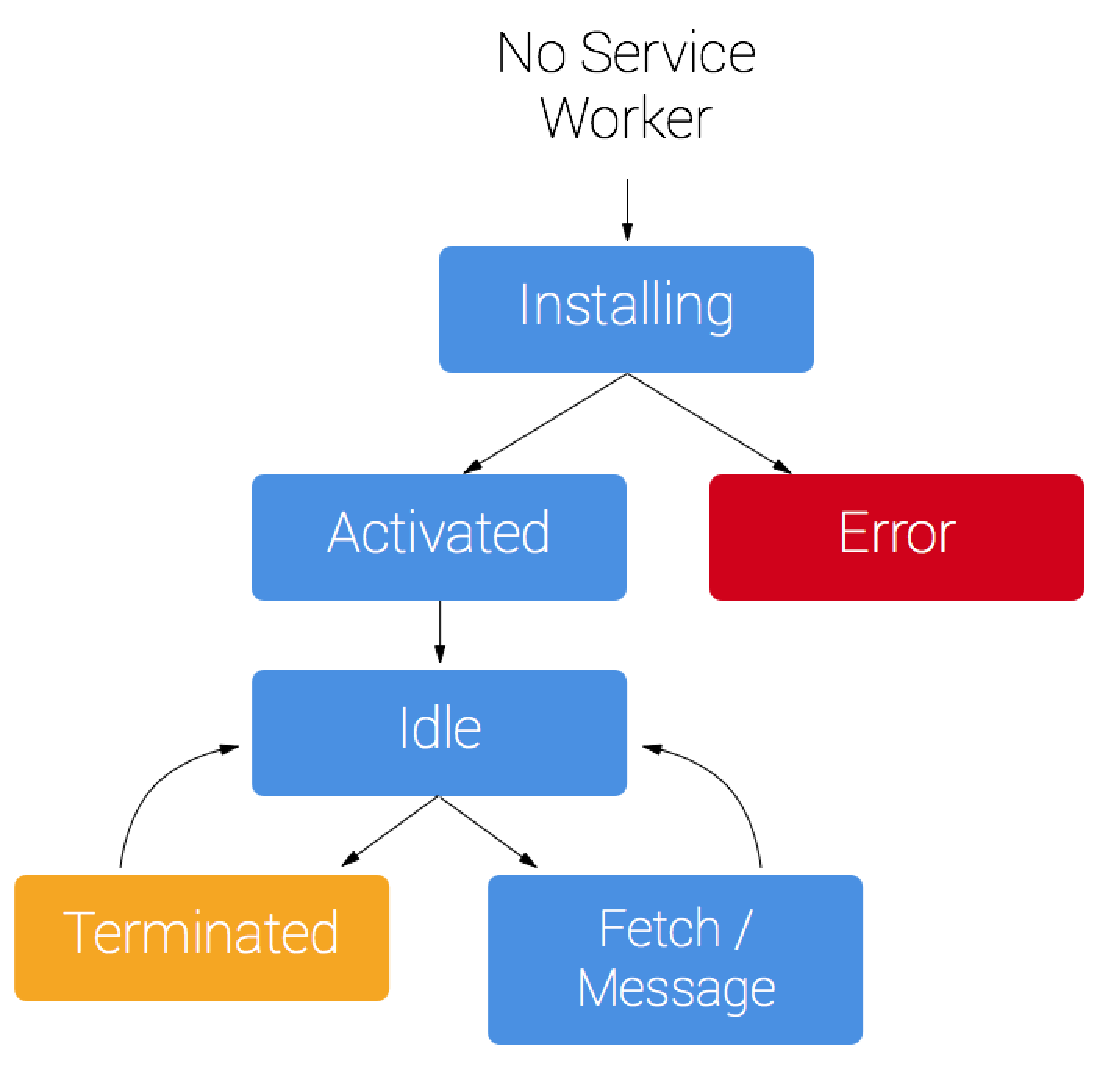
\includegraphics[width=0.8\textwidth]{figures/sw-lifecycle}
	\caption[Lebenszyklus eines Service Workers]{Lebenszyklus eines Service Workers\footnote{https://developers.google.com/web/fundamentals/primers/service-workers/}}
	\label{fig:swLifecycle}
\end{figure}
Nachdem ein Service Worker registriert wurde, befindet er sich im Zustand der Installation. Während der Installation werden häufig Inhalte in den Cache geladen. Wurde der Service Worker erfolgreich installiert, wird er aktiviert. Ab diesem Punkt kann er Requests über das Fetch Event abfangen. Um Arbeitsspeicher zu sparen, wird der Service Worker terminiert, falls er keine Fetch oder Message Events empfängt. Dies hat zur Folge, dass ein Service Worker sich nicht auf den globalen Zustand verlassen kann, sondern stattdessen seinen Zustand auf die IndexedDb ausgelagert werden muss.



%register
%activate
%
%clients.claim

%https://developers.google.com/web/fundamentals/primers/service-workers/ (bild)
%https://developer.mozilla.org/de/docs/Web/API/Service_Worker_API/Using_Service_Workers

\section{Websockets}


Websockets ist ein auf TCP basierendes Protokoll, das bidirektionale Verbindungen zwischen Server und Webanwendung ermöglicht.\cite{rfcWebsockets} Zum Initiieren einer Verbindung wird ein Handshake durchgeführt, der vom Client angestoßen werden muss. Dazu wird wie bei HTTP der Port 80 verwendet. Der Server antwortet bei erfolgreichem Handshake mit dem HTTP Status code 101. Nachdem der Client eine Websocket-Verbindung zum Server aufgebaut hat, ist es dem Server anders als bei HTTP möglich, ohne vorherige Anfrage des Clients Daten an ihn zu senden. Um eine Abwärtskompatibilität zu gewährleisten, werden ähnliche Header wie bei HTTP verwendet.

Neben dem unverschlüsseltem URI-Schema definiert das RFC6455\cite{rfcWebsockets} auch das verschlüsselte Schema wss. Da sehr wenig Daten-Overhead bei der Kommunikation besteht, eignen sich Websockets insbesondere für Anwendungen, die eine geringe Latenz benötigen. Websockets werden von allen modernen Browsern unterstützt.

%bidirektionale verbindung zwischen server und Webanwendung
%auf tcp basierendes protokoll
%very little data overhead needs to be exchanged to send messages. This means a low latency communication.
%WebSockets are great for real-time and long-lived communications.
%
%
%client öffnet verbindung danach kann der server ohne vorherige aktion des cients daten senden
%
% zwei neue URI-Schemata, ws: für unverschlüsselte, und wss: für verschlüsselte Verbindungen.
% 
% handshake zur initierung der verbindung
%  wie http über port 80
%  ähnlicher header --> abwärtskompatibel
%  server antwortet mit http status 101
%  
%WebSockets are supported by all modern browsers.

\section{IP-Adressen}
Eine IP-Adresse ist ein eindeutiger Bezeichner für Computer in einem Netzwerk. Jedem Computer in einem Netzwerk wird eine eindeutige IP-Adresse zugewiesen, über die der Computer adressierbar ist. Dadurch ist der Computer für andere erreichbar. Sie wird benötigt, um ein Routing vom Sender zum Empfänger zu ermöglichen. \cite{www}
\subsection{Aufbau von IP-Adressen}
IPv4 wurde im Jahr 1981 durch das RFC 791\cite{rfc791} definiert und besteht aus einer 32-stelligen Binärzahl, wodurch maximal 4.294.967.296 Adressen dargestellt werden können. Zur besseren Lesbarkeit werden IPv4-Adressen meist dezimal in vier Blöcken dargestellt. IP-Adressen bestehen aus einem Netz- und einem Hostanteil. Mit dem Netzanteil wird das Teilnetz beschrieben, in dem sich das Gerät befindet, während der Hostanteil das Gerät identifiziert. Durch eine Subnetzmaske wird festgelegt, welcher Teil der IP-Adresse Host- und welcher Netzanteil ist. Alle Bits, die in der Subnetzmaske 1 sind, legen den Netzanteil fest - alle Bits, die 0 sind, den Hostanteil.

\begin{table}
\begin{center}
\begin{tabular}{|r|l|l|}
	\hline
	IP-Adresse & 145.574.322. & 5 \\ \hline
	Subnetzmaske & 255.255.255. & 0 \\ \hline
	& Netzanteil & Hostanteil \\
	\hline
\end{tabular}
\caption{Beispiel einer IP-Adresse mit Subnetzmaske}
\end{center}
\end{table}


Aufgrund der stark ansteigenden Zahl an Geräten, die mit dem Internet verbunden sind, ist der Adressbereich der IPv4 Adressen nicht mehr ausreichend. 1998 entwickelte der ITFE deshalb einen neuen Standard. IPv6 verwendet 128 anstatt der 32 Bits zur Darstellung von IP-Adressen. Dadurch ist es möglich, 2$^{32}$ Geräte abzubilden. IPv6 wird meist als vier Oktette hexadezimal dargestellt. Zur Unterscheidung von Host- und Netzanteil werden Präfixlängen angegeben.  

\subsection{Network Address Translation (NAT)}
Mithilfe von NAT können mehrere Geräte über dieselbe öffentliche IP-Adresse über das Internet verbunden werden. Dadurch ist es möglich, trotz des begrenzten Adressraums von IPv4 mehr Geräte mit dem Internet zu verbinden. Dazu werden die IP Adress Header -Felder der Datenpakete verändert.\cite{rfc-nat}

\section{Ruby on Rails}
Ruby on Rails ist ein in Ruby geschriebenes Opensource-Webframework. Zentraler Ansatz der Entwicklung des Frameworks ist es, Software-Entwicklern zu erleichtern, Webanwendungen zu schreiben. Die Philosophie des Frameworks beinhaltet zwei Prinzipien\cite{ror-guide}:

\textbf{Don't Repeat Yourself(DRY):}
Jede Information und Funktionalität soll genau eine Repräsentation im System haben. Dadurch soll erreicht werden, dass die Software einfacher zu warten, über­sicht­licher und fehlerfreier wird.
 
\textbf{Convention over Configuration:}
Um die Entwicklung für den Programmierer zu erleichtern, werden Annahmen getroffen und Standard-Einstellungen festgelegt. Diese lassen sich zwar durch die Entwickler ändern, unterscheiden sich zu Beginn eines Projektes aber noch nicht. So werden z.B. auch Vereinbarungen über die Benennung von Methoden und Klassen getroffen (Naming Conventions).

\section{Turbolinks}
Turbolinks\footnote{https://github.com/turbolinks/turbolinks} ist eine Javascript-Bibliothek zur Beschleunigung der Navigation auf Internetseiten. Klickt ein Nutzer auf einen Link, wird der Seitenabruf unterbrochen und stattdessen mit AJAX geladen. Anschließend überprüft Turbolinks, welche Teile der Seite sich verändert haben und rendert nur diese Elemente. Dadurch entsteht ein flüssigeres Nutzererlebnis, da Teile der Seite bestehen bleiben und nicht ersetzt werden. Da nachgeladene Ressourcen, die sich bei der Navigation nicht ändern, nicht erneut geladen werden müssen, beschleunigt sich die Ladezeit. Javascript-Skripts müssen nicht neu geladen werden, sondern bleiben in ihrem vorherigen Zustand bestehen, da kein kompletter Pageload vorgenommen werden muss.

\section{Single Page Applications}

Unter Single Page Applications (SPA) versteht man Webanwendungen, bei denen der Client aus einem einzigen HTML-Dokument besteht.\cite{spa-def} Inhalte werden meist dynamisch mit AJAX oder Websocket nachgeladen. Sie bieten sich für Anwendungen mit hoher Nutzerzahl an, da der Aufwand der HTML-Renderings vom Server auf den Client verlagert wird. Da das Backend zumeist nur Daten ausliefert, wird die Entwicklung nativer Clients für Mobilgeräte vereinfacht, da zumeist das Backend wiederverwendet werden kann.

\section{Redis}
Bei Redis handelt es sich um einen In-Memory-Datenstrukturspeicher der als LRU-Cache, Datenbank oder Message Broker verwendet werden kann.\footnote{https://redis.io/} Redis ist ein Opensource-Projekt und  wird von Redis Labs gesponsert. Jede gespeicherte Datenstruktur ist über einen Key abrufbar.

Unter anderem unterstützt Redis folgende Datentypen:
Set:
Bei Sets handelt es sich um Mengen, die Strings beinhalten könne, wobei jeder String nur einmal pro Set vorkommt. Hinzufügen von Elementen, Löschen von Elementen und das Prüfen, ob ein Element in einem Set vorhanden ist, passieren in konstanter Zeit. (O(1))\cite{redis-set}

Strings:
Redis Strings sind binary safe, d.h., sie können jegliche Daten, z.B. auch Bilddaten, enthalten. Strings können auch als atomare Zähler verwendet werden. Dazu stellt Redis Kommandos zum Inkrementieren oder Subtrahieren von Strings bereit.

List:
Listen enthalten eine geordnete Liste von Strings in der Reihenfolge, in der sie hinzugefügt wurden. Elemente können sowohl vorne als auch hinten in die Liste eingefügt werden.

\section{HTTP Live-Streaming - HLS}
Beim HTTP Live-Streaming\cite{hls-sdt} werden konventionelle Webserver zur Auslieferung der Videosegmente verwendet. Das Video wird in einzelne Segmente zerlegt, die jeweils einen Teil des Videos enthalten. Diese Segmente werden über HTTP an die Nutzer verteilt. Dadurch ist es möglich, auf bestehende Verteilungsstrukturen zurückzugreifen. Indem für jedes Segment unterschiedliche Qualitäten vorgehalten werden, ist es möglich, die Qualität des Video an die Bandbreite des Nutzers anzupassen, während es abgespielt wird.
